\documentclass[border=10pt]{standalone}
\usepackage{tikz}
\usetikzlibrary{shapes.geometric}
\usetikzlibrary{arrows.meta,arrows}
\begin{document}

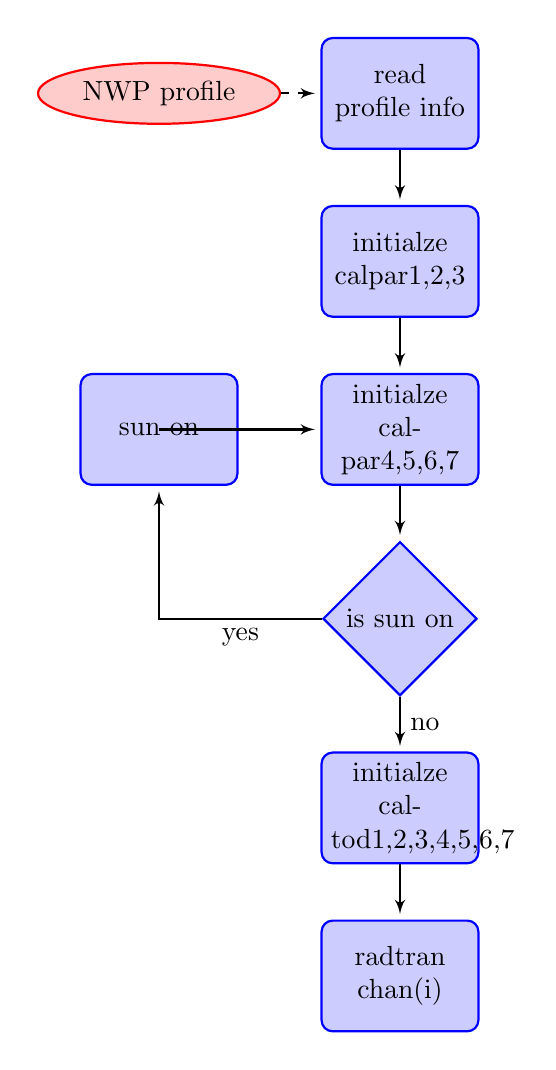
\begin{tikzpicture}
[auto,
decision/.style={diamond, draw=blue, thick, fill=blue!20,
text width=4.5em,align=flush center,
inner sep=1pt},
block/.style ={rectangle, draw=blue, thick, fill=blue!20,
text width=5em,align=center, rounded corners,
minimum height=4em},
line/.style ={draw, thick, -latex',shorten >=2pt},
cloud/.style ={draw=red, thick, ellipse,fill=red!20,
minimum height=2em}]
\matrix [column sep=5mm,row sep=7mm]
{
% row 1  has three thingies
\node [cloud]  (nwp)  {NWP profile}; &
\node [block] (init) {read profile info}; & \\
% row 2 has a blank thingy and another thingy and a blank thigy
& \node [block] (calparA)    {initialze calpar1,2,3}; & \\
% row 3 has two thingyies and a blank thingy
\node [block] (yessun)       {sun on}; & 
\node [block] (calparB)    {initialze calpar4,5,6,7}; & \\
% row 4
& \node [decision] (checksun1) {is sun on}; &  \\
% row 5
& \node [block] (caltod)  {initialze caltod1,2,3,4,5,6,7}; & \\
% row 6
& \node [block] (radtrans) {radtran chan(i)}; & \\
};
\begin{scope}[every path/.style=line]
\path [dashed] (nwp) -- (init);
\path (init) -- (calparA);
\path (calparA) -- (calparB);
\path (yessun) |- (calparB);
\path (checksun1) -| node [near start] {yes} (yessun);
\path (calparB) -- (checksun1);
\path (checksun1) -- node {no} (caltod);
\path (caltod) -- (radtrans);
%\path [dashed] (calparB) |- node [near start] {sun init} (caltod);
\end{scope}
\end{tikzpicture}

\end{document} 
